\documentclass[11pt]{article}

\usepackage[margin=1in]{geometry}
\usepackage{amsmath}
\usepackage{amssymb}
\usepackage{booktabs}
\usepackage{graphicx}
\usepackage{xcolor}
\usepackage[font=small,labelfont=bf]{caption}
\usepackage{titlesec}
\usepackage{enumitem}
\usepackage[colorlinks=true,linkcolor=black,urlcolor=blue!60!black,citecolor=black]{hyperref}

\definecolor{good}{HTML}{2E7D32}
\definecolor{bad}{HTML}{B3282D}
\definecolor{warn}{HTML}{B26A00}
\newcommand{\yes}{\textcolor{good}{\textbf{reproduced}}}
\newcommand{\no}{\textcolor{bad}{\textbf{not reproduced}}}
\newcommand{\dprime}{d'}
\newcommand{\dd}{\Delta d'}
\newcommand{\dc}{\Delta c}
\newcommand{\dg}{\ensuremath{^\circ}}

\titleformat{\section}{\normalfont\large\bfseries}{\thesection}{0.6em}{}
\titleformat{\subsection}{\normalfont\normalsize\bfseries}{\thesubsection}{0.6em}{}

\title{\vspace{-1.2cm}\textbf{Does the $d_{\mathrm{mem}}{=}128$ dual-stream pair reproduce the\\
Luo--Maunsell sensitivity/criterion dissociation?}\\[2mm]
\large A frozen-policy SDT assay of two partially trained, cost-rescued policies}
\author{Experiment report}
\date{18 August 2026}

\begin{document}
\maketitle
\vspace{-0.7cm}

\begin{abstract}
\noindent Two RunPod training runs of the $d_{\mathrm{mem}}{=}128$ dual-stream
counterphased sensitivity design were terminated early for cost and their
checkpoints rescued at iterations 18{,}799 (high-priority location~0) and 15{,}849
(location~3) of a 20{,}000-iteration contract. Re-running the repository's frozen-policy
signal-detection assay on both policies gives a clear split verdict. The
\emph{sensitivity} component of the Luo--Maunsell (LM) effect is \yes: the counterphased
difference-in-differences in $\dprime$ is positive with a bootstrap CI excluding zero at
all three evaluated difficulties ($\dd_{\mathrm{DiD}} = +0.23$ to $+0.32$). The
\emph{specificity} component --- criterion invariance --- is \no: the criterion
cross-effect is $\dc_{\mathrm{DiD}} \approx +0.23$, whose CI extends past the
preregistered $\pm 0.2$ equivalence bound, so the strict dissociation test fails.
The central new finding is \emph{why} it fails. The observed criterion shift matches,
to within $0.03$, the reward-optimal criterion implied by the task's own
hit:correct-rejection ratios ($0.7$ at the high-priority location versus $1.1$ at the
low). The agents are not miscalibrated; they are sitting on the optimum that the reward
schedule specifies. Because that optimum is $\dc = 0.452/\dprime$, the $\pm 0.2$ target
is unreachable unless $\dprime \gtrsim 2.26$ at both locations, whereas these policies
achieve $\dprime = 1.67$--$2.10$. Doubling recurrent width did improve criterion
\emph{calibration} --- the $d_{\mathrm{mem}}{=}64$ parent overshot the reward optimum by
$2.1\times$, while this pair brackets it --- but no amount of memory or training can
satisfy a specificity target that the uncorrected reward table forbids. The design must
be criterion-titrated before it can test the LM dissociation.
\end{abstract}

\section{Scope, and what ``the LM results'' means here}

``LM'' is read throughout as Luo \& Maunsell (2015, \emph{Neuron} 86:1182--1188), the
source protocol named in the task module \texttt{envs/luo2015.py}. The effect being
chased is their dissociation between two components of attention: a spatial manipulation
that changes detection \emph{sensitivity} ($\dprime$) should leave the decision
\emph{criterion} ($c$) essentially unchanged, and vice versa.

The repository encodes this as two preregistered targets
(\texttt{latest\_full\_battery\_manifest.json}):

\begin{itemize}[leftmargin=1.4em,itemsep=1pt]
  \item \textbf{sensitivity lineage} --- positive counterphased $\dprime$
        difference-in-differences, with the criterion cross-effect inside an
        equivalence bound of $|\dc| \le 0.2$;
  \item \textbf{criterion lineage} --- negative counterphased $c$
        difference-in-differences, with the $\dprime$ cross-effect inside the same bound.
\end{itemize}

\noindent\textbf{Scope limit.} Both rescued runs are \emph{sensitivity} cells. The
experiment package states plainly that ``criterion cells are unsupported'' in this
design. This report can therefore address only the first half of the dissociation.
Establishing a double dissociation would additionally require the criterion lineage,
which was never run in this family. Nothing below should be read as evidence about the
criterion-manipulation half.

A second scope limit is inherited from the experiment manifest itself, whose
\texttt{claim\_scope} field reads

\begin{quote}\ttfamily\footnotesize
memory\_capacity\_followup\_in\_uniform\_change\_noisy\_\\
memory\_extension\_not\_direct\_luo\_maunsell\_replication
\end{quote}

\noindent and which warns that the ``fixed H:CR ratios directly pressure criterion.''
That warning turns out to be the whole story (Section~\ref{sec:reward}).

\section{Provenance of the two runs}

Both pods ran the identical launch contract from

\begin{quote}\ttfamily\footnotesize
experiments/luo2015\_episodic/fresh\_dualstream\_dmem128\_grid2\_\\
memnoise0075\_gamma100\_bc000\_curriculum\_sensitivity\_runpod
\end{quote}

\noindent differing only in the
\texttt{--high-loc} flag. Fresh seed-0 initialisation, 2$\times$2 token grid, xLSTM cell with
\texttt{crossattn1} feedback, separate actor and critic streams with independent
recurrent state and independent JEPA branches at coefficient $0.5$ each, teacher EMA
$0.996$, $\gamma = 1.0$, mnemonic-noise SD $0.075$, sensory jitter $5\dg$, BC
coefficient $0$, reward scale $1/3$, shrinking-$\theta$ curriculum from $65\dg$
(window 1000 valid SDT trials, threshold $0.85$, step $3\dg$, floor $8\dg$).

\begin{table}[h]
\centering\small
\caption{Status of the two runs at rescue. The contract was 20{,}000 iterations; neither
reached it. ``Last observed'' is the final successful probe by the local monitoring
watchdog, after the rescue snapshot was taken.}
\label{tab:provenance}
\begin{tabular}{lrr}
\toprule
 & \textbf{high-priority loc 0} & \textbf{high-priority loc 3} \\
\midrule
Pod ID                        & \texttt{5ic3h9bmujytt2} & \texttt{kmmqwwmd4uaweu} \\
Rescued checkpoint iteration  & 18{,}799 & 15{,}849 \\
Metrics rows captured         & 18{,}840 & 15{,}888 \\
Last iteration observed       & 19{,}516 & 15{,}986 \\
Fraction of contract          & 94\% & 79\% \\
Terminal curriculum $\theta$  & $47\dg$ & $38\dg$ \\
Final rolling correct rate    & 0.805 & 0.823 \\
Best rolling correct rate     & 0.898 & 0.890 \\
Checkpoint SHA-256 verified   & yes & yes \\
\bottomrule
\end{tabular}
\end{table}

Two honest caveats about the artifacts:

\begin{enumerate}[leftmargin=1.4em,itemsep=2pt]
\item \textbf{The checkpoints are partial.} The repository's terminal validators
(\texttt{validate\_checkpoint}, \texttt{validate\_curriculum\_checkpoint}) assert
\texttt{iter == 19999} and were therefore bypassed. Every other element of the
measurement contract was kept. Results below are frozen-policy measurements of
non-terminal policies, not terminal replication evidence.
\item \textbf{A later checkpoint was lost.} The snapshot was taken at 04:44~UTC; the runs
continued during download and verification, and the watchdog last saw a checkpoint at
iteration 19{,}499 for the loc-0 cell before the pods were terminated at approximately
04:56~UTC. Roughly 700 further iterations of the loc-0 lineage exist only as
now-deleted pod state. The analysis uses iteration 18{,}799.
\end{enumerate}

The evaluation imports the model and environment definitions from the \emph{rescued pod
source tree}, not the working copy: \texttt{model.py}, \texttt{paper\_encoder.py},
\texttt{ppo.py} and \texttt{train\_rl.py} in the local repository have been modified since
launch, whereas \texttt{envs/luo2015.py}, \texttt{envs/base.py} and
\texttt{luo2015\_analysis/luo2015\_core.py} are byte-identical to the deployed versions.

\section{Task and measurement contract}

Two Gabors sit at diametrically opposed cells (0 = top-left, 3 = bottom-right) of a
2$\times$2 grid, each with an independent orientation drawn from
$\mathrm{Uniform}[0\dg,180\dg)$. There is no value cue. After a delay one location is
tested, either unchanged or offset by a signed change drawn from
$\mathrm{Uniform}(-\theta,+\theta)$. A declaration during the first-test window
(frames 3--4) is a hit or a false alarm; withholding is verified by a required
declaration to a guaranteed-changed second test at frame 6, and failures of that check
are excluded from the SDT denominators, as in the paper. $\dprime = z(\mathrm{HR}) -
z(\mathrm{FA})$ and $c = -\tfrac{1}{2}\,[z(\mathrm{HR}) + z(\mathrm{FA})]$, with rates
clamped to $[1/2N, 1-1/2N]$.

Measurement followed the repository assay exactly: one deterministic balanced trial bank
shared by both policies, 2{,}000 trials per change-status per location (8{,}000 trials per
bank), trained mnemonic noise enabled, sampled categorical policy actions, and
5{,}000-draw bootstrap confidence intervals. Evaluation ran on the exact rescued source
under PyTorch 1.13.1/CUDA on an RTX 3070; all six rescued checkpoints were verified to
deserialise with finite weights before use.

Because the two lineages stalled at different curriculum depths, three evaluation
branches were run: each policy at its own terminal $\theta$, and both policies on shared
banks at $\theta \in \{38\dg, 47\dg, 50\dg\}$. The shared-bank branches are what make
the counterphased difference-in-differences interpretable, and $\theta = 50\dg$ matches
the difficulty at which the $d_{\mathrm{mem}}{=}64$ parent was measured.

The counterphased estimand is
\begin{equation}
\mathrm{DiD}(m) \;=\; \tfrac{1}{2}\Big[\big(m_0 - m_3\big)\big|_{\text{high}=0}
\;-\; \big(m_0 - m_3\big)\big|_{\text{high}=3}\Big],
\label{eq:did}
\end{equation}
which cancels any location-intrinsic bias shared by the two policies. Positive
$\mathrm{DiD}(\dprime)$ means each policy discriminates better at \emph{its own}
high-priority location.

\section{Results}

\subsection{Learning and curriculum depth}

Both runs learned and both stalled (Figure~\ref{fig:training}). The loc-0 lineage
descended to $\theta = 47\dg$ by iteration 5{,}839 and then advanced no further through
iteration 19{,}516. The loc-3 lineage descended faster and further, reaching $41\dg$ by
iteration 4{,}451 and $38\dg$ at 12{,}577. Neither approached the $8\dg$ floor, and both
hovered near, but mostly below, the $0.85$ advancement threshold --- rolling correct
rates settled around $0.80$--$0.82$. The primary hypothesis of the design (that doubling
$d_{\mathrm{mem}}$ ``improves \ldots\ curriculum depth'') is not supported by these
partial runs: the deeper lineage here, $38\dg$, is the one that ran \emph{fewer}
iterations.

\begin{figure}[h]
\centering
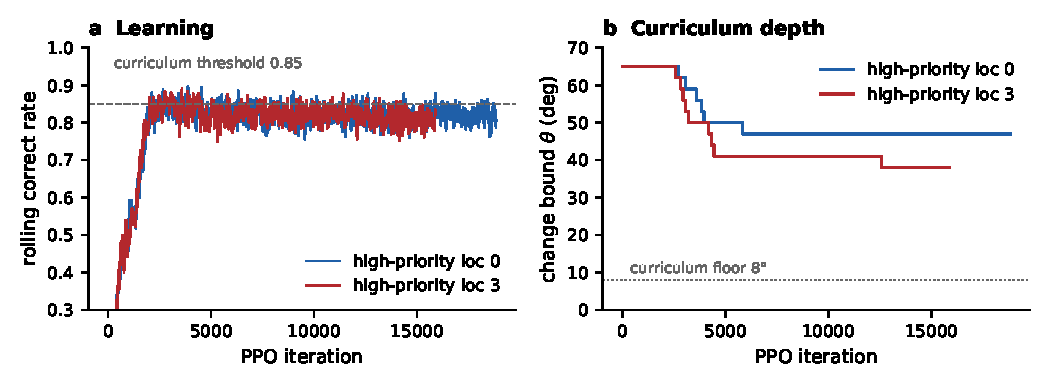
\includegraphics[width=\textwidth]{figs/fig_training.pdf}
\caption{Training trajectories of the two rescued runs. (a) Rolling correct rate.
(b) Curriculum change bound $\theta$, a step function decremented by $3\dg$ whenever a
1000-trial window exceeds 0.85 correct. Both lineages stall well above the $8\dg$ floor.}
\label{fig:training}
\end{figure}

\subsection{Per-location signal detection}

Table~\ref{tab:sdt} gives the frozen-policy SDT decomposition at each policy's own
terminal $\theta$. Counterphasing is \emph{sign-correct in both lineages and for both
metrics}: each policy has both higher $\dprime$ and higher $c$ at its own high-priority
location. The magnitudes, however, are strikingly asymmetric --- the loc-0 lineage shows
$\dd = +0.433$ while the loc-3 lineage shows only $\dd = +0.053$ (CI includes zero).
This is not a difficulty artifact: on the shared $\theta = 47\dg$ bank the same gap
persists ($+0.460$ versus $+0.172$), as it does at $50\dg$ ($+0.348$ versus $+0.114$).
The positive group-level sensitivity effect is thus carried disproportionately by one of
the two lineages, which is a real weakness of the counterphase in this pair.

\begin{table}[h]
\centering\small
\caption{Frozen-policy SDT at each policy's own terminal $\theta$, trained mnemonic noise,
sampled actions, 2{,}000 trials per change-status per location. $\ast$ marks the
high-priority (condition) location. The $d_{\mathrm{mem}}{=}64$ parent is the terminal
loc-3 checkpoint measured at $\theta = 50\dg$.}
\label{tab:sdt}
\begin{tabular}{llrrrrr}
\toprule
\textbf{Policy} & \textbf{loc} & $\dprime$ & $c$ & HR & FA & $n$/status \\
\midrule
$d_{\mathrm{mem}}{=}128$ loc 0 & 0$\ast$ & 2.104 & 0.373 & 0.751 & 0.077 & 1999 \\
(iter 18{,}799, $\theta{=}47\dg$)   & 3       & 1.671 & 0.093 & 0.771 & 0.177 & 2000 \\[2pt]
$d_{\mathrm{mem}}{=}128$ loc 3 & 0       & 2.007 & 0.409 & 0.724 & 0.079 & 2000 \\
(iter 15{,}849, $\theta{=}38\dg$)   & 3$\ast$ & 2.059 & 0.534 & 0.690 & 0.059 & 2000 \\[2pt]
$d_{\mathrm{mem}}{=}64$ loc 3  & 0       & 1.625 & 0.062 & 0.774 & 0.191 & 2000 \\
(iter 19{,}999, $\theta{=}50\dg$)   & 3$\ast$ & 2.049 & 0.551 & 0.682 & 0.058 & 1999 \\
\bottomrule
\end{tabular}
\end{table}

Repeating the own-$\theta$ branch with mnemonic noise \emph{disabled} changes almost
nothing ($\dd = +0.445$ and $+0.087$; $\dc = +0.295$ and $+0.126$), so neither the
sensitivity effect nor the criterion shift is an artifact of noise injection at
measurement time.

\subsection{The counterphased test}

\begin{table}[h]
\centering\small
\caption{Counterphased difference-in-differences (Equation~\ref{eq:did}) on shared trial
banks, with 5{,}000-draw bootstrap CIs. The sensitivity target is met at every difficulty;
the specificity target is missed at every difficulty. The final column is the
reward-optimal criterion shift predicted from the task's own reward table
(Section~\ref{sec:reward}), computed from the measured per-location $\dprime$.}
\label{tab:did}
\begin{tabular}{lccc c}
\toprule
 & $\dd_{\mathrm{DiD}}$ (CI) & $\dc_{\mathrm{DiD}}$ (CI) & strict & $\dc$ predicted \\
\midrule
$\theta = 38\dg$ & $+0.239$ $[+0.140,+0.335]$ & $+0.227$ $[+0.179,+0.276]$ & \textcolor{bad}{fail} & $+0.237$ \\
$\theta = 47\dg$ & $+0.316$ $[+0.216,+0.420]$ & $+0.241$ $[+0.190,+0.291]$ & \textcolor{bad}{fail} & $+0.212$ \\
$\theta = 50\dg$ & $+0.231$ $[+0.135,+0.330]$ & $+0.228$ $[+0.179,+0.277]$ & \textcolor{bad}{fail} & $+0.213$ \\
\bottomrule
\end{tabular}
\end{table}

The sensitivity result is robust: positive point estimate, CI excluding zero, at all
three difficulties (Figure~\ref{fig:did}). The specificity result fails, though narrowly
in absolute terms --- the criterion CIs \emph{straddle} the bound (lower limits
$0.179$--$0.190$ lie inside $\pm 0.2$; upper limits $0.276$--$0.291$ lie outside), so the
equivalence test, which requires the entire interval inside the band, is not satisfied.
The point estimates sit only $0.03$--$0.04$ above the bound.

\begin{figure}[h]
\centering
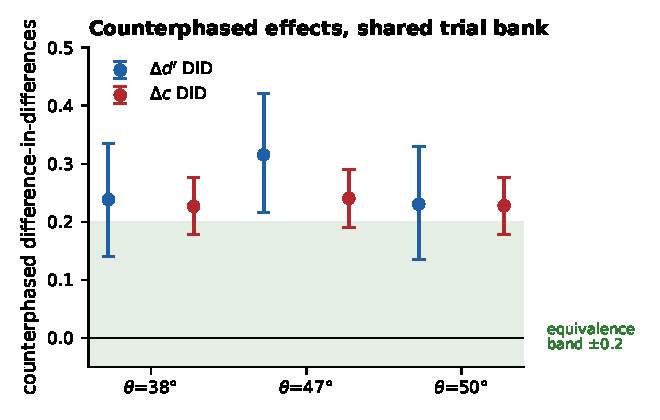
\includegraphics[width=0.62\textwidth]{figs/fig_did.pdf}
\caption{Counterphased difference-in-differences at three difficulties. The sensitivity
effect (blue) clears zero everywhere. The criterion cross-effect (red) sits just above
the $\pm 0.2$ equivalence band (green) everywhere.}
\label{fig:did}
\end{figure}

\subsection{The criterion shift is reward-optimal, not a failure of learning}
\label{sec:reward}

The sensitivity session assigns the high-priority location a mean reward of 5 with a
hit:correct-rejection ratio of $0.7$, and the low-priority location a mean reward of 1
with a ratio of $1.1$. Expanding the ratios gives per-location payoffs of
$R_{\mathrm{hit}} = 4.118$, $R_{\mathrm{CR}} = 5.882$ at the high location and
$R_{\mathrm{hit}} = 1.048$, $R_{\mathrm{CR}} = 0.952$ at the low. Misses and false alarms
pay zero and $P(\mathrm{change}) = 0.5$ exactly, so the reward-optimal likelihood-ratio
criterion at a location is simply
\begin{equation}
\beta^{\ast} \;=\; \frac{P(\text{no change})}{P(\text{change})}\cdot
\frac{R_{\mathrm{CR}} - R_{\mathrm{FA}}}{R_{\mathrm{hit}} - R_{\mathrm{miss}}}
\;=\; \frac{R_{\mathrm{CR}}}{R_{\mathrm{hit}}} \;=\; \frac{1}{\text{H:CR ratio}},
\end{equation}
and for equal-variance Gaussian SDT the corresponding criterion is
$c^{\ast} = \ln \beta^{\ast} / \dprime$. The high location therefore \emph{should} be run
more conservatively than the low one, by
\begin{equation}
\Delta \ln \beta^{\ast} \;=\; \ln(1/0.7) - \ln(1/1.1) \;=\; 0.452 .
\label{eq:dlnbeta}
\end{equation}

This is the crux. The reward table \emph{mandates} a criterion difference; it is not a
nuisance the agent could learn away. Converting Equation~\ref{eq:dlnbeta} into the
criterion units of the equivalence bound, using each policy's measured per-location
$\dprime$, predicts $\dc_{\mathrm{DiD}} = +0.213$ to $+0.237$ across the three
difficulties. The observed values are $+0.227$, $+0.241$, $+0.228$ --- agreement to
within $0.03$ (Table~\ref{tab:did}, Figure~\ref{fig:reward}). These policies are sitting
essentially exactly where the reward schedule tells them to sit.

\begin{figure}[h]
\centering
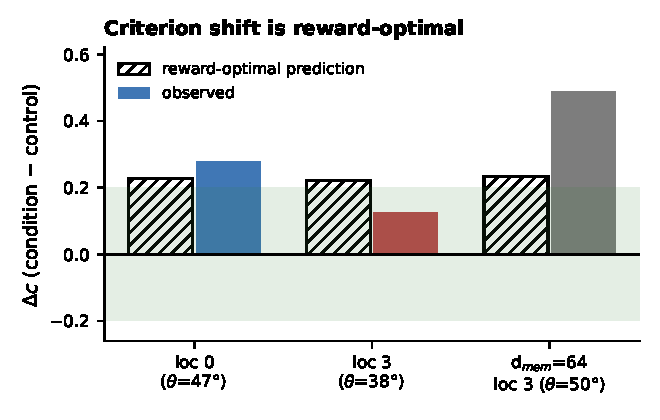
\includegraphics[width=0.62\textwidth]{figs/fig_reward_optimal.pdf}
\caption{Observed criterion shift against the reward-optimal prediction
$\dc^{\ast} = \ln\beta^{\ast}/\dprime$ computed from the measured per-location $\dprime$.
The $d_{\mathrm{mem}}{=}64$ parent overshoots the optimum by $2.1\times$; the
$d_{\mathrm{mem}}{=}128$ pair brackets it ($1.23\times$ and $0.57\times$). The optimum
itself lies just outside the $\pm 0.2$ band.}
\label{fig:reward}
\end{figure}

Two consequences follow.

\textbf{First, the specificity target is unreachable at the sensitivity these agents
achieve.} Setting $c^{\ast} \le 0.2$ with a common $\dprime$ at both locations requires
\begin{equation}
\dprime \;\ge\; \frac{0.452}{0.2} \;=\; 2.26 ,
\end{equation}
whereas the measured values are $1.67$--$2.10$ (Table~\ref{tab:sdt}). A perfectly
reward-rational agent would fail this experiment's specificity test. No increase in
memory width, training length or curriculum depth fixes that, because the requirement is
a property of the payoff matrix, not of the policy --- unless the agent were pushed to
$\dprime > 2.26$, at which point the same reward table would become compatible with the
bound.

\textbf{Second, doubling the recurrent width did improve criterion calibration, which is
a real and previously untested effect.} The $d_{\mathrm{mem}}{=}64$ parent produced
$\dc = +0.489$ against a reward-optimal $+0.233$ --- an overshoot of $2.1\times$, i.e.\ it
was substantially \emph{more} conservative at its high-value location than payoff
maximisation warrants. The $d_{\mathrm{mem}}{=}128$ policies give $1.23\times$ (loc 0) and
$0.57\times$ (loc 3), bracketing the optimum, with the counterphased average landing on it.
On the matched $\theta = 50\dg$ bank the loc-3 cell moved from $\dc = +0.489$ at
$d_{\mathrm{mem}}{=}64$ to $\dc = +0.142$ at $d_{\mathrm{mem}}{=}128$, i.e.\ from far
outside the equivalence band to comfortably inside it --- but its sensitivity effect
shrank in step, from $\dd = +0.425$ to $+0.114$.

\begin{figure}[h]
\centering
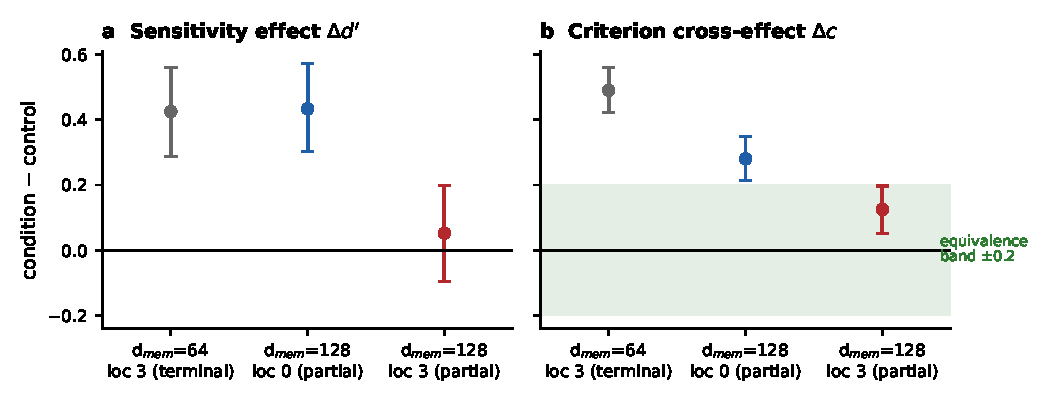
\includegraphics[width=\textwidth]{figs/fig_contrasts.pdf}
\caption{Per-policy condition-minus-control contrasts with bootstrap CIs.
(a) The sensitivity effect is large in the loc-0 lineage and near zero in the loc-3
lineage. (b) The criterion cross-effect. The $d_{\mathrm{mem}}{=}64$ parent sits far
outside the equivalence band; both $d_{\mathrm{mem}}{=}128$ policies are closer to it,
and the loc-3 policy is inside it.}
\label{fig:contrasts}
\end{figure}

\section{Verdict}

\begin{table}[h]
\centering\small
\caption{Effect-by-effect verdict against the preregistered targets.}
\label{tab:verdict}
\begin{tabular}{p{5.6cm}p{3.0cm}p{6.0cm}}
\toprule
\textbf{Target} & \textbf{Outcome} & \textbf{Evidence} \\
\midrule
Positive counterphased $\dprime$ DiD
 & \textcolor{good}{reproduced}
 & $+0.23$ to $+0.32$, CI excludes zero at $\theta = 38, 47, 50\dg$ \\[3pt]
Sign-correct counterphasing in both lineages
 & \textcolor{good}{reproduced}
 & Both policies have higher $\dprime$ \emph{and} higher $c$ at their own high-priority location \\[3pt]
Symmetric counterphase
 & \textcolor{warn}{partial}
 & $\dd = +0.433$ (loc 0) versus $+0.053$ (loc 3) at own $\theta$; gap persists at matched difficulty \\[3pt]
Criterion cross-effect inside $|\dc| \le 0.2$
 & \textcolor{bad}{not reproduced}
 & $\dc_{\mathrm{DiD}} \approx +0.23$, CI upper limit $0.276$--$0.291$ \\[3pt]
Strict behavioural dissociation
 & \textcolor{bad}{not achieved}
 & Fails at every difficulty and for every individual policy \\[3pt]
LM \emph{double} dissociation
 & \textcolor{bad}{not testable here}
 & Criterion lineage unsupported in this design; only sensitivity cells were run \\
\bottomrule
\end{tabular}
\end{table}

In one sentence: \textbf{the sensitivity half of the LM effect reproduced, the criterion
specificity did not, and the reason it did not is that this reward schedule makes
criterion invariance incompatible with reward-rational behaviour at the sensitivity
these agents reach.}

The falsifier written into the experiment manifest --- ``the sensitivity gain remains
coupled to a criterion shift outside the preregistered equivalence band'' --- is
therefore met, and the $d_{\mathrm{mem}}$ capacity hypothesis is not rescued by these
runs. But the falsifier fires for a reason that is external to the manipulation under
test, so it should be read as a verdict on the \emph{design}, not on memory capacity.

\section{What to change before running this again}

\begin{enumerate}[leftmargin=1.5em,itemsep=3pt]
\item \textbf{Titrate the reward table.} Hold the hit:correct-rejection ratio
\emph{equal} across locations and vary only the mean reward, so that
$\Delta \ln \beta^{\ast} = 0$ and the reward-optimal $\dc$ is zero by construction. The
sensitivity manipulation then acts through value/effort allocation without mandating a
criterion difference, and $|\dc| \le 0.2$ becomes a meaningful test rather than an
arithmetic impossibility. This is the single change with the largest effect on whether
the experiment can succeed.
\item \textbf{Report the reward-optimal criterion alongside the observed one} in the
standard assay output. Both this run and its parent are far more interpretable as
ratios to $c^{\ast}$ than as raw $\dc$ values; without it, the $d_{\mathrm{mem}}{=}64$
result reads as a simple failure rather than as a $2.1\times$ overshoot.
\item \textbf{Fix the curriculum stall before adding capacity.} Both lineages parked
well above the $8\dg$ floor at $\approx 0.80$--$0.82$ correct against a $0.85$ threshold.
Sensitivity is the binding constraint on specificity here --- $\dprime \ge 2.26$ would by
itself bring the reward-optimal $\dc$ inside the band --- so effort spent reaching deeper
$\theta$ is also effort spent making the specificity test passable.
\item \textbf{Run the criterion lineage.} Without it there is no double dissociation to
claim, only one half of one.
\item \textbf{Investigate the lineage asymmetry.} A $8\times$ difference in $\dd$ between
two runs differing only in \texttt{--high-loc} is large enough to warrant seeds beyond
seed 0 before the counterphased DiD is trusted as a group estimate.
\end{enumerate}

\section{Limitations}

\begin{itemize}[leftmargin=1.4em,itemsep=2pt]
\item \textbf{Partial checkpoints.} 94\% and 79\% of the training contract. The
terminal-iteration validators were bypassed. The comparison against the
$d_{\mathrm{mem}}{=}64$ parent is therefore partial-versus-terminal, which flatters
neither side in a predictable direction.
\item \textbf{Single seed.} Seed 0 only, one policy per condition location. All CIs are
trial-resampling intervals within a fixed pair of policies; they do not cover
seed-to-seed variability, which the lineage asymmetry suggests is substantial.
\item \textbf{Different terminal difficulties.} The two lineages stalled at $47\dg$ and
$38\dg$. This is handled by the shared-bank branches, and the DiD is stable across
$38$--$50\dg$, but no shared bank is simultaneously ``terminal'' for both policies.
\item \textbf{Parent comparison is single-cell.} The $d_{\mathrm{mem}}{=}64$ reference is
one loc-3 checkpoint evaluated on its own bank at $\theta = 50\dg$ with a different
evaluation seed; there is no $d_{\mathrm{mem}}{=}64$ loc-0 cell, so no parent DiD exists.
\item \textbf{Equal-variance SDT.} $c^{\ast} = \ln\beta^{\ast}/\dprime$ assumes the
equal-variance Gaussian model. Unequal variance would shift the predicted values
somewhat, though not enough to move a $0.45$ log-odds mandate inside a $0.2$ band at
$\dprime \approx 2$.
\item \textbf{Not a neural replication.} This is a behavioural SDT analogue. Nothing here
speaks to the V4 modulation results that motivate the original paper.
\end{itemize}

\section{Artifacts}

All inputs and outputs are under the rescue root\\
\texttt{C:\textbackslash Users\textbackslash jomor\textbackslash runpod\_rescue\textbackslash 20260817}.
\texttt{loc0/} and \texttt{loc3/} hold the rescued run directories (checkpoint, full
\texttt{metrics.csv}, supervisor log, manifests, launch and deployment contracts, pod
provenance including \texttt{pip freeze}), \texttt{eval\_tree/} holds the exact pod source
plus the assay driver \texttt{run\_partial\_sdt.py} and its output
\texttt{results/partial\_sdt\_results.json}, and \texttt{report/} holds
\texttt{analyze\_and\_plot.py}, \texttt{analysis\_summary.json}, the figures and this
document. The assay is reproducible with

\begin{quote}\small
\texttt{python run\_partial\_sdt.py --trials 2000 --bootstrap-draws 5000}\\
\texttt{\phantom{python run\_partial\_sdt.py} --common-thetas 38 47 50}
\end{quote}

\noindent Checkpoints were written under NumPy~2 and require the
\texttt{numpy.\_core} module alias when loaded under NumPy~1; the driver installs it.

\end{document}
